\documentclass[tikz,border=10pt]{standalone}
\usepackage{tikz}
\usetikzlibrary{scopes}
\usepackage{verbatim}
\usepackage{xcolor}
\usetikzlibrary{calc,angles,patterns,quotes}


\definecolor{aqua}{rgb}{0.0, 1.0, 1.0}
\definecolor{babyblue}{rgb}{0.54, 0.81, 0.94}

\newcommand\wcol{babyblue!60}

\begin{document}
  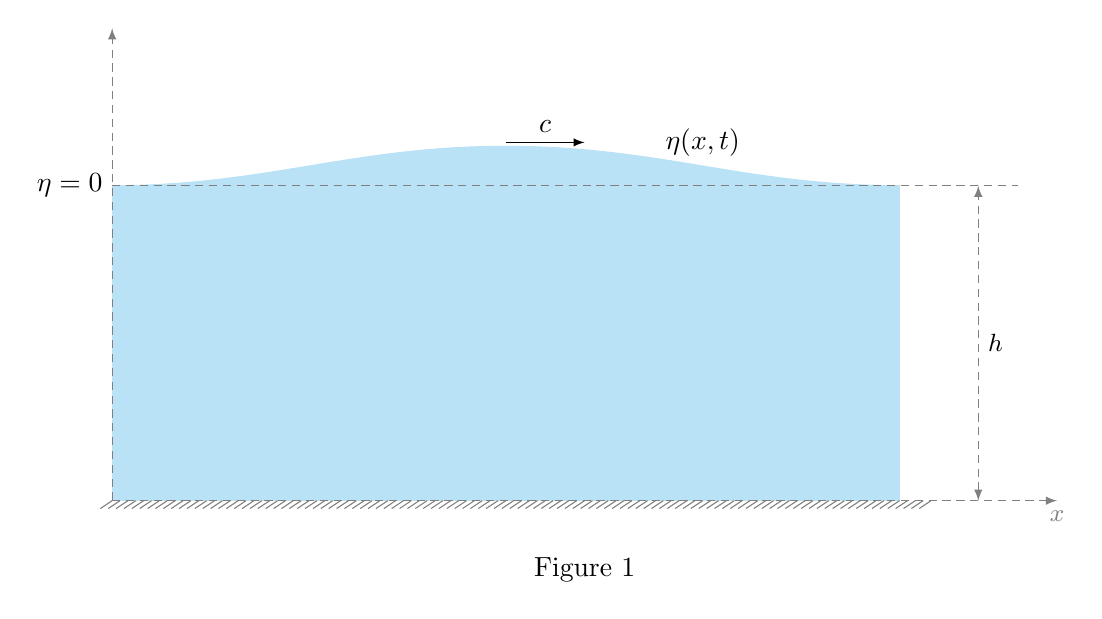
\begin{tikzpicture}[
      axis/.style={densely dashed,gray,font=\small},
      vector/.style={>=latex,draw=black,fill=black}
    ]
    \filldraw[fill=\wcol, draw=\wcol] (-5, 2) -- (5, 2) -- (5, -2) -- (-5, -2) -- cycle;
    \draw[>=latex, axis, ->] (-5, -2) -- ++(0, 6);


    \draw[>=latex, axis, ->] (-5, -2) -- ++(12, 0) node[below]{$x$};

    \filldraw [fill=\wcol,draw=\wcol] (-5, 2) to[out=0, in=180] (0, 2.5) to[out=0, in=180] node[above]{$\eta(x, t)$} (5, 2);
    \draw[vector, ->] (0, 2.55) -- node[above]{$c$} ++(1, 0);

    \draw[>=latex, axis, <->] (6, -2) -- node[right,color=black]{$h$} ++(0, 4);
    \draw[>=latex, axis] (-5, 2) -- ++(11.5, 0);
    \node[left, anchor=east] at (-5, 2) {$\eta=0$};

    \foreach \x in {-5,-4.9,...,5.5}{
      \draw[axis, solid] (\x, -2) -- ++(-0.15, -0.1);
    }


    \node[below, anchor=north] at (1, -2.6) {Figure 1};
  \end{tikzpicture}



  %% simpler plot
  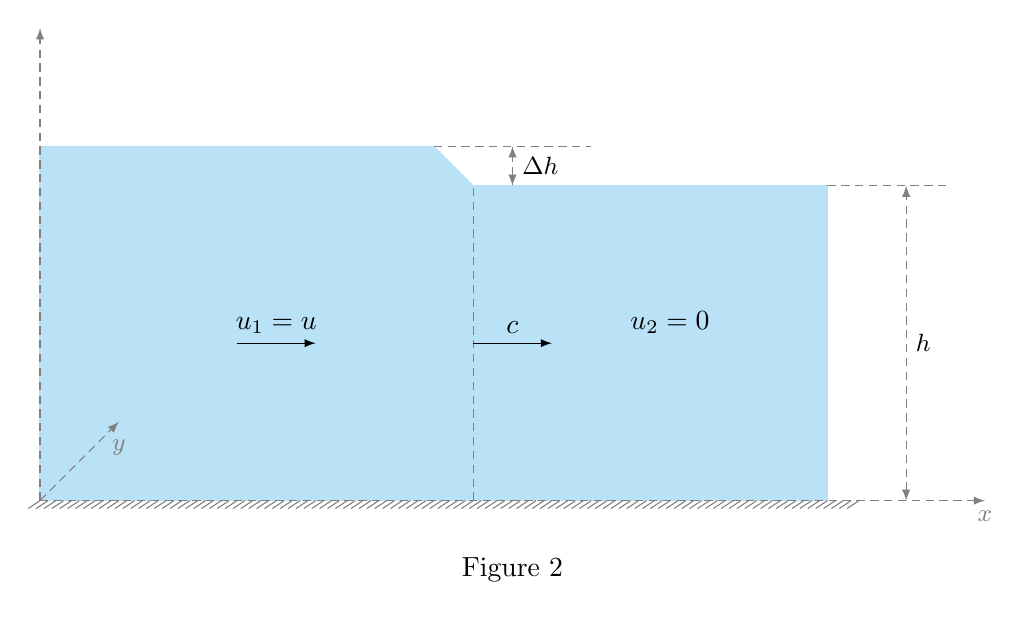
\begin{tikzpicture}[
    axis/.style={densely dashed,gray,font=\small},
    vector/.style={>=latex,draw=black,fill=black}
  ]
    \filldraw[fill=\wcol, draw=\wcol] (-5, 2) -- (5, 2) -- (5, -2) -- (-5, -2) -- cycle;
    \filldraw[fill=\wcol, draw=\wcol] (-5, 2.5) -- (0, 2.5) -- (0.5, 2) -- (-5, 2) -- cycle;
    \draw[>=latex, axis, ->] (-5, -2) -- ++(0, 6);
    \draw[>=latex, axis, ->] (-5, -2) -- ++(12, 0) node[below]{$x$};

    \draw[>=latex, axis, <->] (6, -2) -- node[right,color=black]{$h$} ++(0, 4);
    \draw[axis] (5, 2) -- ++(1.5, 0);
    \draw[axis] (0, 2.5) -- ++(2, 0);
    \draw[>=latex, axis, <->] (1, 2) -- node[right,color=black]{$\Delta h$} ++(0, 0.5);

    \draw[axis] (0.5, -2) -- ++(0, 4);

    \draw[>=latex, axis, ->] (-5, -2) -- ++(1, 1) node[below=3] {$y$};


    \draw[vector, ->] (-2.5, 0) -- node[above]{$u_1 = u$} ++(1, 0);
    \draw[vector, ->] (0.5, 0) -- node[above]{$c$} ++(1, 0);
    \path (2.5, 0) -- node[above]{$u_2 = 0$} ++(1, 0);

    \foreach \x in {-5,-4.9,...,5.5}{
      \draw[axis, solid] (\x, -2) -- ++(-0.15, -0.1);
    }


    \node[below, anchor=north] at (1, -2.6) {Figure 2};


  \end{tikzpicture}

\end{document}
